% This is a basic Math Paper

\documentclass[11pt]{article}

% Preamble

\usepackage[margin=1in]{geometry}
\usepackage{amsfonts, amsmath, amssymb}
\usepackage{fancyhdr, float, graphicx}
\usepackage[utf8]{inputenc} % Required for inputting international characters
\usepackage[T1]{fontenc} % Output font encoding for international characters
\usepackage{fouriernc} % Use the New Century Schoolbook font
\usepackage[nottoc, notlot, notlof]{tocbibind}
\usepackage{url}

% Header and Footer
\pagestyle{fancy}
\fancyhead{}
\fancyfoot{}
\fancyhead[L]{\textit{\Large{Assignment 2}}}
%\fancyhead[R]{\textit{something}}
\fancyfoot[C]{\thepage}
\renewcommand{\footrulewidth}{1pt}



% Other Doc Editing
% \parindent 0ex
%\renewcommand{\baselinestretch}{1.5}

\begin{document}
	
	\begin{titlepage} 
		\centering 
		
		%---------------------------NAMES-------------------------------
		
		\huge\textsc{
			MIT World Peace University
		}\\
	
		\vspace{0.75\baselineskip} % space after Uni Name
		
		\LARGE{
			Engineering Physics\\
			First Year B. Tech, Trimester 3\\
			Academic Year 2021-22
		}
		
		\vfill % space after Sub Name
		
		%--------------------------TITLE-------------------------------
		
		\rule{\textwidth}{1.6pt}\vspace*{-\baselineskip}\vspace*{2pt}
		\rule{\textwidth}{0.6pt}
		\vspace{0.75\baselineskip} % Whitespace above the title
		
		
		
		\huge{\textsc{
				Schrodinger's Cat, Quantum Entanglement, Quantum Superposition and Qubits
			}} \\
		
		
		
		\vspace{0.5\baselineskip} % Whitespace below the title
		\rule{\textwidth}{0.6pt}\vspace*{-\baselineskip}\vspace*{2.8pt}
		\rule{\textwidth}{1.6pt}
		
		\vspace{1\baselineskip} % Whitespace after the title block

		%--------------------------SUBTITLE --------------------------	
			
		\LARGE\textsc{
			Physics Assignment 2
		} % Subtitle or further description
		\vfill
		
		%--------------------------AUTHOR-------------------------------
		
		Prepared By
		\vspace{0.5\baselineskip} % Whitespace before the editors
		
		\Large{
			109054. Krishnaraj Thadesar
						
			Division 9 Batch I3
		}
		
		
		\vspace{0.5\baselineskip} % Whitespace below the editor list
		\today

	\end{titlepage}
	
\tableofcontents
\clearpage

\section{Introduction}
In the following assignment, we will try to understand some more fundamental concepts surrounding quantum Mechanics, of which the first one
is Schrodinger's Cat. To know what a cat has to do with the foundations of the universe and Reality as we know it, we will have to look
at a little bit of history surrounding the birth of Quantum Mechanics Itself. Understanding the Schrodinger's Cat requires us to have an understanding of all the other topics on this assignment, so in the process of figuring the cat out, we will go through them one by one, as one leads to another. 

\subsection{The Quantum War}


The Post World War I Era (1922). Everything was changing. The rise and fall of world powers, the rise and fall of culture, revolutions, and people. In the midst of it all was the rise of Modern physics itself. Around this time the experiment that would shock physicists globally, and for decades to come, was done in Bell Labs, New Jersey.\\

Just like we saw the interference pattern with light, they did an double slit experiment with electron beams, and noticed the same pattern as seen by classical waves during diffraction. This meant, the electrons have to be a wave. First light which was thought of as waves, starts behaving like particles, and now electrons which were thought of as particles, are starting to behave like waves? So the electrons were interfering with each other? \\

And it doesnt even end there. What if instead of a beam of electrons, you fired one electron at a time? then surely it wouldnt be able to interfere with other electrons right, coz they arent even there? Well it turns out you \textit{still} see the pattern. That basically means, that every single electron behaves like a wave. And this wave interferes with \textit{itself}, to contribute to the interference pattern. \\

\subsection{The Copenhagen Interpretation}
Neils Bohr, is the leader on this side of the war. He is a firm believer that the quantum world is vastly different from the real one, and bizarre as well. So bizarre, in fact, that when an electron is shot, it actually \textit{goes through both slits at the same time, and its wave then after passing through, it can actually simultaneously exist at all the points of the interference pattern, and only when we look at it, or make a detection, or place a screen is when you get to know where it actually is.} This is when your wave of probabilty collapses. This is known as the copenhagen interpretation, given copenhagen is the capital of Norway, and Neils Bohr was Dutch.  \\

Ofcourse, The other side of the war, was lead by Einstein and Schrodinger himself. They hated this. Einstein said that there is no way we dont know where the electron is unless we look at it. The moon doesnt just stop existing while I am not looking at it. These 2 men argued with each other for the next 10 years, until at the end the copenhagen interpretation was finally accepted by the scientific community, and is a the standard accepted even today, as it continues to stand the test of time. \\

Bohr here describes a \textit{Superposition} of the electron's quantum State. To understand what that means, we have to understand what is superposition.


\begin{figure}
	\begin{center}
		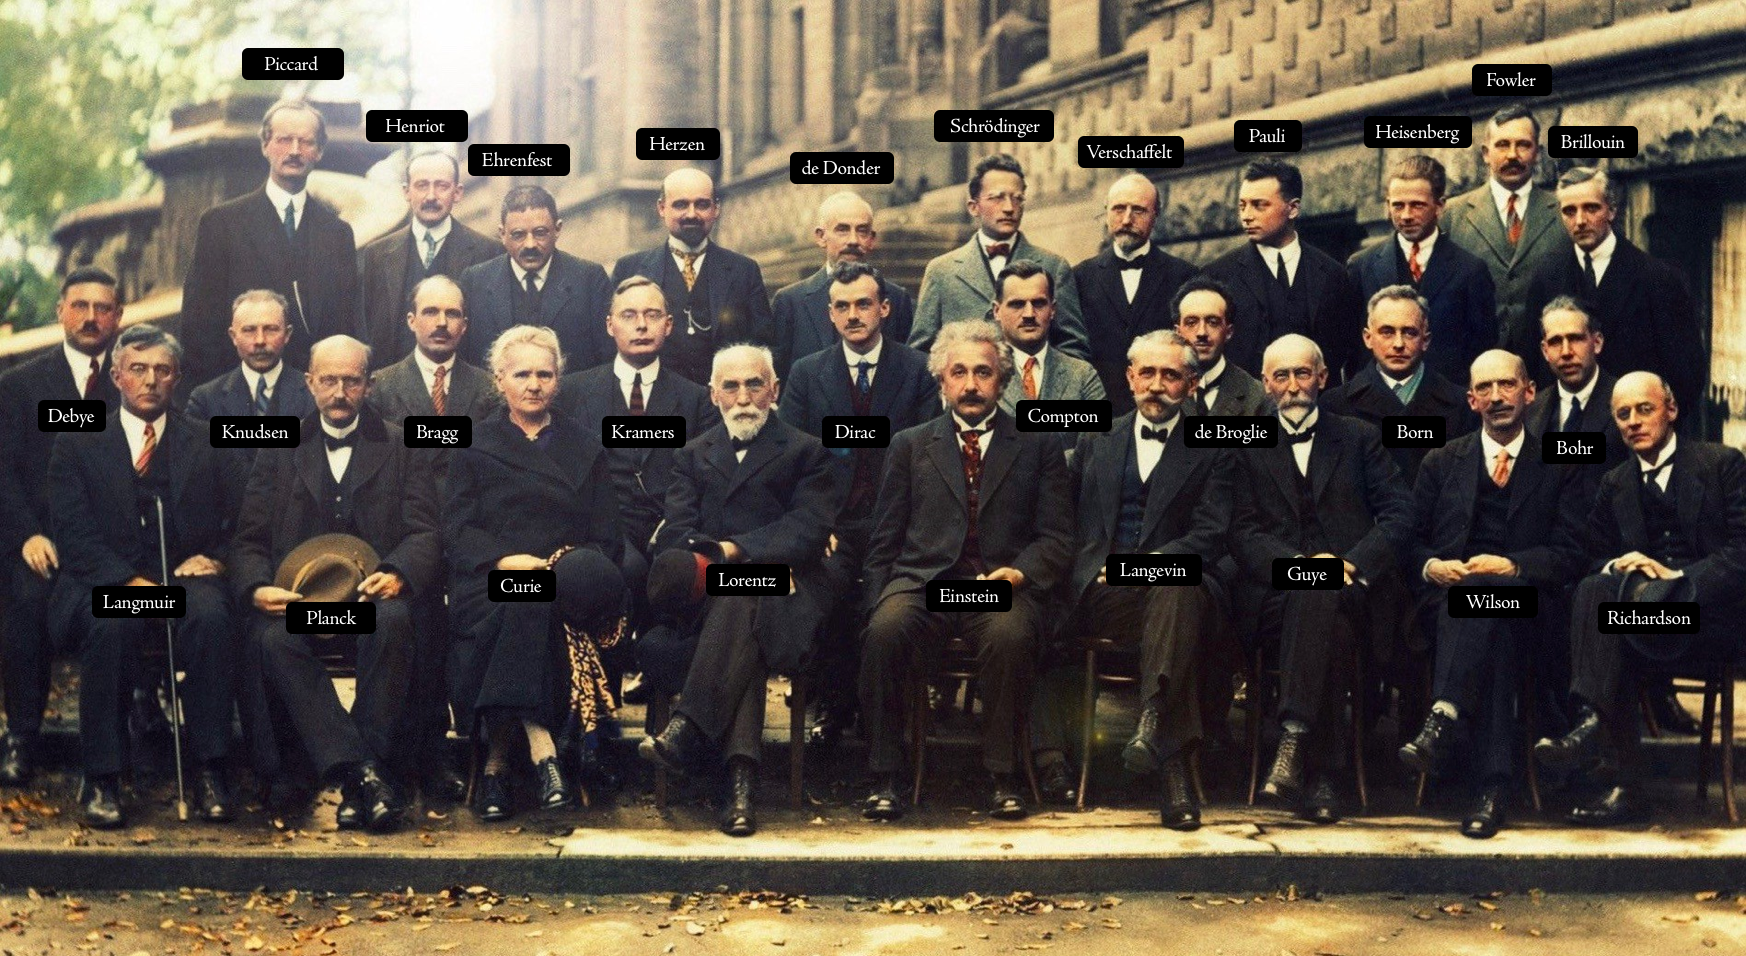
\includegraphics[scale=0.25]{1935 Quantum Mechanics Conference.png}
		\caption{October 1927 Fifth Solvay International Conference on Electrons and Photons, where the world’s most notable physicists met to discuss the newly formulated quantum theory. The leading figures were Albert Einstein and Niels Bohr. You can notice Heisenberg's one of the only person smiling. This is coz his theory was accepted, while Einsteins was assumed wrong. }
	\end{center}
\end{figure}
\section{Quantum Superposition}
Quantum superposition is a fundamental principle of quantum mechanics. It states that, much like waves in classical physics, any two (or more) quantum states can be added together ("superposed") and the result will be another valid quantum state; and conversely, that every quantum state can be represented as a sum of two or more other distinct states. Mathematically, it refers to a property of solutions to the Schrödinger equation; since the Schrödinger equation is linear, any linear combination of solutions will also be a solution.\\

An example of a physically observable manifestation of the wave nature of quantum systems is the interference peaks from an electron beam in a double-slit experiment. The pattern is very similar to the one obtained by diffraction of classical waves.\\

The principle of quantum superposition states that if a physical system may be in one of many configurations—arrangements of particles or fields—then the most general state is a combination of all of these possibilities, where the amount in each configuration is specified by a complex number.\\

For example, if there are two configurations labelled by 0 and 1, the most general state would be

$${\displaystyle c_{0}{\mid }0\rangle +c_{1}{\mid }1\rangle }$$

where the coefficients are complex numbers describing how much goes into each configuration.\\


\textit{The general principle of superposition of quantum mechanics applies to the states [that are theoretically possible without mutual interference or contradiction] ... of any one dynamical system. It requires us to assume that between these states there exist peculiar relationships such that whenever the system is definitely in one state we can consider it as being partly in each of two or more other states. The original state must be regarded as the result of a kind of superposition of the two or more new states, in a way that cannot be conceived on classical ideas. Any state may be considered as the result of a superposition of two or more other states, and indeed in an 
infinite number of ways. Conversely, any two or more states may be superposed to give a new state} - Paul Dirac

\begin{figure}
	\centering
	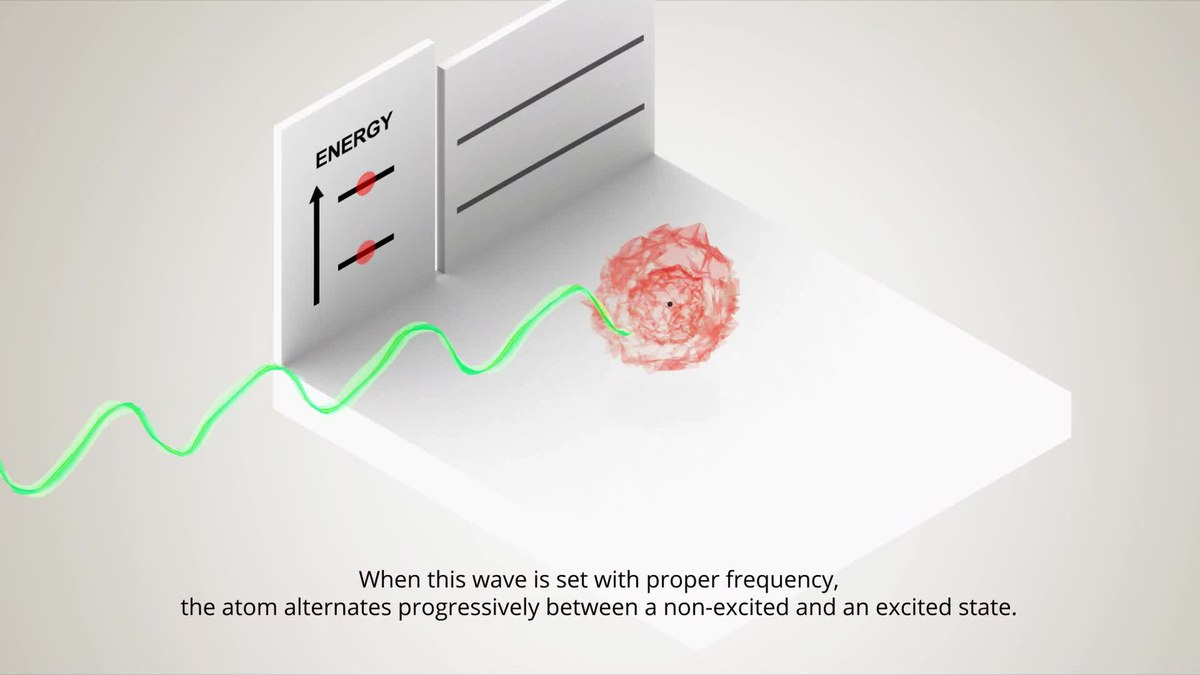
\includegraphics[scale = 0.3]{superposition.jpg}
	\caption{An Example of how an atom would be in an excited as well as ground state at the same time, unless observed. }
\end{figure}


\section{Qubits}

Another example of Quantum Superposition is a quantum logical qubit state, as used in quantum information processing, which is a quantum superposition of the "basis states" $ {\displaystyle |0\rangle } $ and $ {\displaystyle |1\rangle } $  \\


In quantum computing, a qubit or quantum bit is a basic unit of quantum information—the quantum version of the classic binary bit physically realized with a two-state device. A qubit is a two-state (or two-level) quantum-mechanical system, one of the simplest quantum systems displaying the peculiarity of quantum mechanics. \\

 
\subsection{Notation}
In quantum mechanics, the general quantum state of a qubit can be represented by a linear superposition of its two orthonormal basis states (or basis vectors). These vectors are usually denoted as $${\displaystyle |0\rangle ={\bigl [}{\begin{smallmatrix}1\\0\end{smallmatrix}}{\bigr ]}} \text{ and } {\displaystyle |1\rangle ={\bigl [}{\begin{smallmatrix}0\\1\end{smallmatrix}}{\bigr ]}}$$They are written in the conventional Dirac—or "bra - ket"—notation; the ${\displaystyle |0\rangle }$  and ${\displaystyle |1\rangle }$ are pronounced "ket 0" and "ket 1", respectively.


\subsection{Qubit States}

A pure qubit state is a coherent superposition of the basis states. This means that a single qubit can be described by a linear combination of ${\displaystyle |0\rangle } $ and ${\displaystyle |1\rangle }$:

$ {\displaystyle |\psi \rangle =\alpha |0\rangle +\beta |1\rangle }$

where $\alpha$ and \(\beta\) are probability amplitudes, that are both complex numbers. When we measure this qubit in the standard basis, according to the born rule, the probability of outcome $ |0\rangle $ with value "0" is ${\displaystyle |\alpha |^{2}} $and the probability of outcome ${\displaystyle |1\rangle }$ with value "1" is ${\displaystyle |\beta |^{2}}$, Because the absolute squares of the amplitudes equate to probabilities, it follows that ${\displaystyle \alpha }$  and ${\displaystyle \beta }$ must be constrained according to the second axiom of probability theory by the equation

$${\displaystyle |\alpha |^{2}+|\beta |^{2}=1.}$$

\begin{figure}
	\centering
	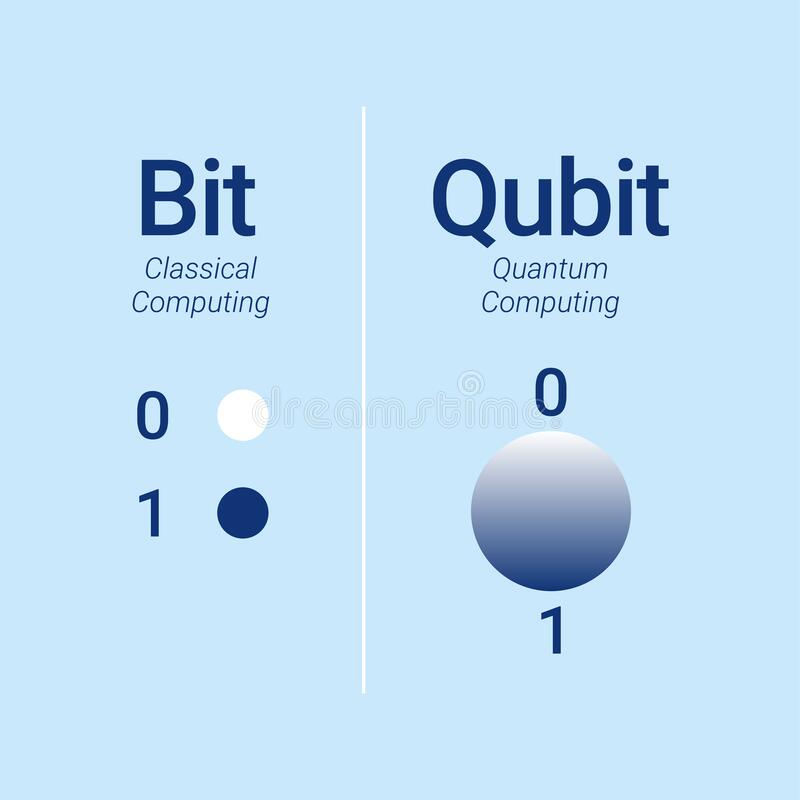
\includegraphics[scale = 0.3]{qbits.jpg}
	\caption{An Example of how an atom would be in an excited as well as ground state at the same time, unless observed. }
\end{figure}

\section{Quantum Entanglement}
Even more surprising than superposition, quantum theory predicts that entities may have correlated fates. That is, the result of a measurement on one photon or atom leads instantaneously to a correlated result when an entangled photon or atom is measured.

For a more intuitive grasp of what we mean by “correlated results,” imagine that two coins could be entangled (there is no known way of doing this with coins, of course). Imagine one is tossing a coin. Careful records show it comes up “heads” about half the time and “tails” half the time, but any one result is unpredictable. Tossing another coin has similar, random results, but surprisingly, the records of the coin tosses show a correlation! When one coin comes up heads, the other coin comes up tails and vice versa. We say that the state of the two coins is entangled. Before the measurement (the toss), the outcome is unknown, but we know the outcomes will be correlated. As soon as either coin is tossed (measured), the fate of tossing the other coin is sealed. We cannot predict in advance what an individual coin will do, but their results will be correlated: once one is tossed, there is no uncertainty about the other.

This imaginary coin tossing is only to give the reader a sense of entanglement. Although one might come up with a classical explanation for these results, multitudes of ingenious experiments have confirmed the existence of entanglement and ruled out any possible classical explanation. Over several decades, physicists have continually refined these experiments to remove loopholes in measurement accuracy or subtle assumptions. All have confirmed the predictions of quantum mechanics.

\subsection{EPR Paradox}
As Einstein, Podolsky and Rosen discovered, entanglement appears instantaneous: Once you have knowledge of one quantum state, you automatically know the quantum state of any entangled particles. In principle, you could place two entangled particles on opposite ends of the galaxy and still have this instantaneous knowledge, which appears to violate the limit of the speed of light.\\

This result is known as the EPR paradox (short for Einstein, Podolsky and Rosen), according to the American Physical Society — an effect Einstein dubbed "spooky action at a distance." He used the paradox as evidence that quantum theory was incomplete. But experiments have repeatedly confirmed that entangled particles do influence each other regardless of distance, and quantum mechanics remains verified to this day.

\subsection{Creating Entangled Particles}

There are many ways to entangle particles. One method is to cool the particles and place them close enough together so that their quantum states (representing the uncertainty in the position) overlap, making it impossible to distinguish one particle from the other.\\

Another way is to rely on some subatomic process, like nuclear decay, that automatically produces entangled particles. According to NASA, it's also possible to create entangled pairs of photons, or particles of light, by either splitting a single photon and generating a pair of photons in the process, or by mixing pairs of photons in a fiber-optic cable.

\section{Schrodinger's Cat}

So that now brings us back to schrodinger's Cat. The many astounding and shocking concepts that we read about so far, were just as bizzare back in the day as they are now.
Schrodinger hated this fact. He could not accept that a quantum state could be in 2 states at the same time. So to prove how ridiculous all of this is, and how incomplete the copenhagen interpretation of quantum mechanics was, he used the Cat Experiment. Instead of disproving the interpretation however, it went on to be a fundamental tool to 
explain quantum mechanics worldwide. \\

Schrödinger wrote:\\

\textit{One can even set up quite ridiculous cases. A cat is penned up in a steel chamber, along with the following device (which must be secured against direct interference by the cat): in a Geiger counter, there is a tiny bit of radioactive substance, so small, that perhaps in the course of the hour one of the atoms decays, but also, with equal probability, perhaps none; if it happens, the counter tube discharges and through a relay releases a hammer that shatters a small flask of hydrocyanic acid. If one has left this entire system to itself for an hour, one would say that the cat still lives if meanwhile no atom has decayed. The first atomic decay would have poisoned it. The psi-function of the entire system would express this by having in it the living and dead cat (pardon the expression) mixed or smeared out in equal parts.\\
It is typical of these cases that an indeterminacy originally restricted to the atomic domain becomes transformed into macroscopic indeterminacy, which can then be resolved by direct observation. That prevents us from so naïvely accepting as valid a "blurred model" for representing reality. In itself, it would not embody anything unclear or contradictory. There is a difference between a shaky or out-of-focus photograph and a snapshot of clouds and fog banks.}\\


Einstein, who was impressed by the ability of the thought experiment to highlight these issues. In a letter to Schrödinger dated 1950, he wrote:\\


\textit{
You are the only contemporary physicist, besides Laue, who sees that one cannot get around the assumption of reality, if only one is honest. Most of them simply do not see what sort of risky game they are playing with reality—reality as something independent of what is experimentally established. Their interpretation is, however, refuted most elegantly by your system of radioactive atom + amplifier + charge of gun powder + cat in a box, in which the psi-function of the system contains both the cat alive and blown to bits. Nobody really doubts that the presence or absence of the cat is something independent of the act of observation.}\\


A commonly held interpretation of quantum mechanics is the Copenhagen interpretation.[10] In the Copenhagen interpretation, a system stops being a superposition of states and becomes either one or the other when an observation takes place. This thought experiment makes apparent the fact that the nature of measurement, or observation, is not well-defined in this interpretation. The experiment can be interpreted to mean that while the box is closed, the system simultaneously exists in a superposition of the states "decayed nucleus/dead cat" and "undecayed nucleus/living cat", and that only when the box is opened and an observation performed does the wave function collapse into one of the two states.\\

\begin{figure}[]
	\centering
	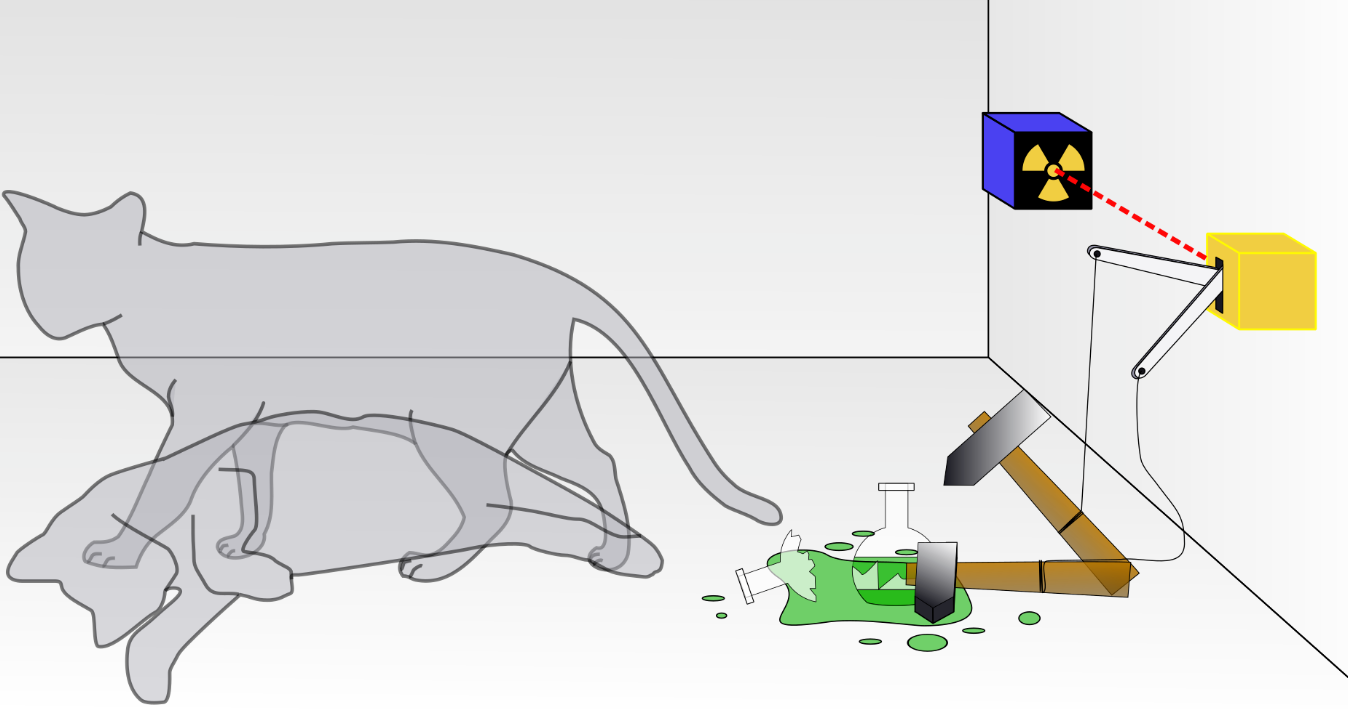
\includegraphics[scale = .3] {cat.png}
	\caption{The Cat, both being dead and alive at the same time. }
\end{figure}
\clearpage
\end{document}